En esta sección, vamos a comprobar empíricamente que nuestro algoritmo tiene una complejidad temporal de $O(n^3*k)$.

En este primer caso utilizamos instancias controladas donde cada casillero tiene una potencia de 1. A su vez, utilizamos un k fijo en cada caso. Probamos con distintos $n$ y obtuvimos el resultado que se puede observar en las figuras debajo.

\begin{figure}[H]
  \begin{minipage}{0.5\linewidth}
    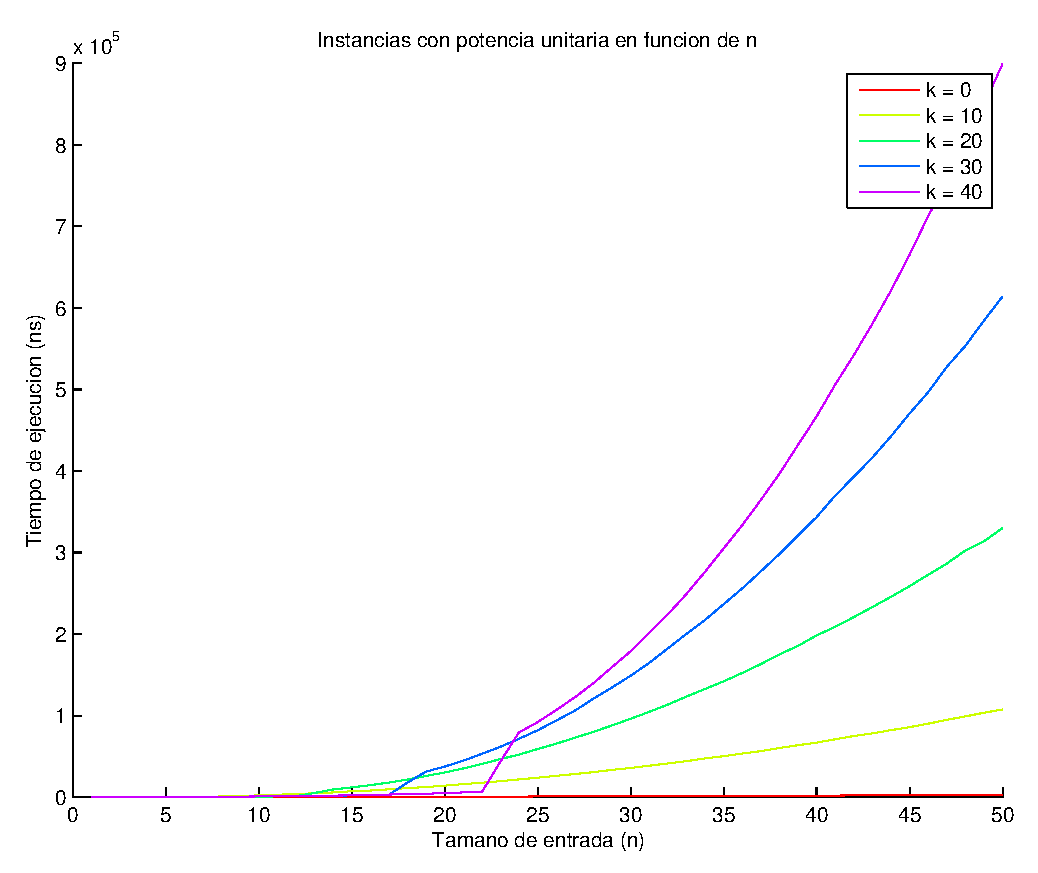
\includegraphics[width=\linewidth]{img/problema3/instancia_p_1_varios_k.eps}
    \caption{Tiempo de ejecución instancia aleatoria}\label{fig:problema3-k}
  \end{minipage}
  \hfill
  \begin{minipage}{0.5\linewidth}
    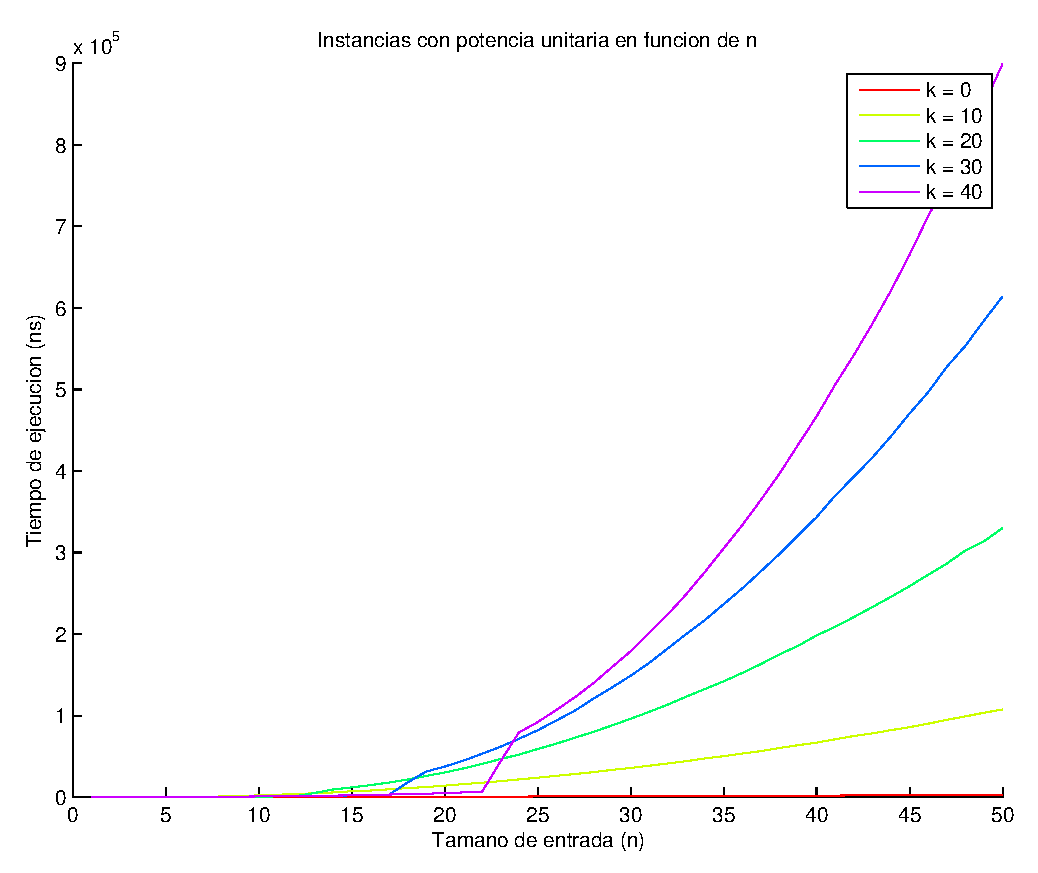
\includegraphics[width=\linewidth]{img/problema3/instancia_p_1_varios_k_div_n2.eps}
    \caption{Idem, dividido por $n^2$}\label{fig:problema3-k-n2}
  \end{minipage}
\end{figure}

En la figura \ref{fig:problema3-k} no podemos notar la complejidad temporal de la función. Por esto, dividimos por $n^2$ y plasmamos ese resultado en la figura \ref{fig:problema3-k-n2}. En esta última figura, vemos claramente que $T(n) / n ^ 2$ es una recta. De esta manera, pudimos comprobar empíricamente que $T(n)$ tiene una complejidad temporal de $O(n^3)$, lo cual demostramos anteriormente.

Observando el gráfico observamos que en los casos donde $k \geq 2*(n-2)$ resolver el problema es trivial y este caso lo cubrimos en el primer ejemplo de la seccion \ref{problema3-descripcion}. Los casos interesantes son cuando $k < 2*(n-2)$. En estos casos, la complejidad del algoritmo se vuelve $O(n^3*k)$ como podemos observar en la figura \ref{fig:problema3-k-n2}.

Luego, realizamos otro experimento: dejamos los n fijos y variamos con distintos k.

\begin{figure}[H]
  \begin{minipage}{0.5\linewidth}
    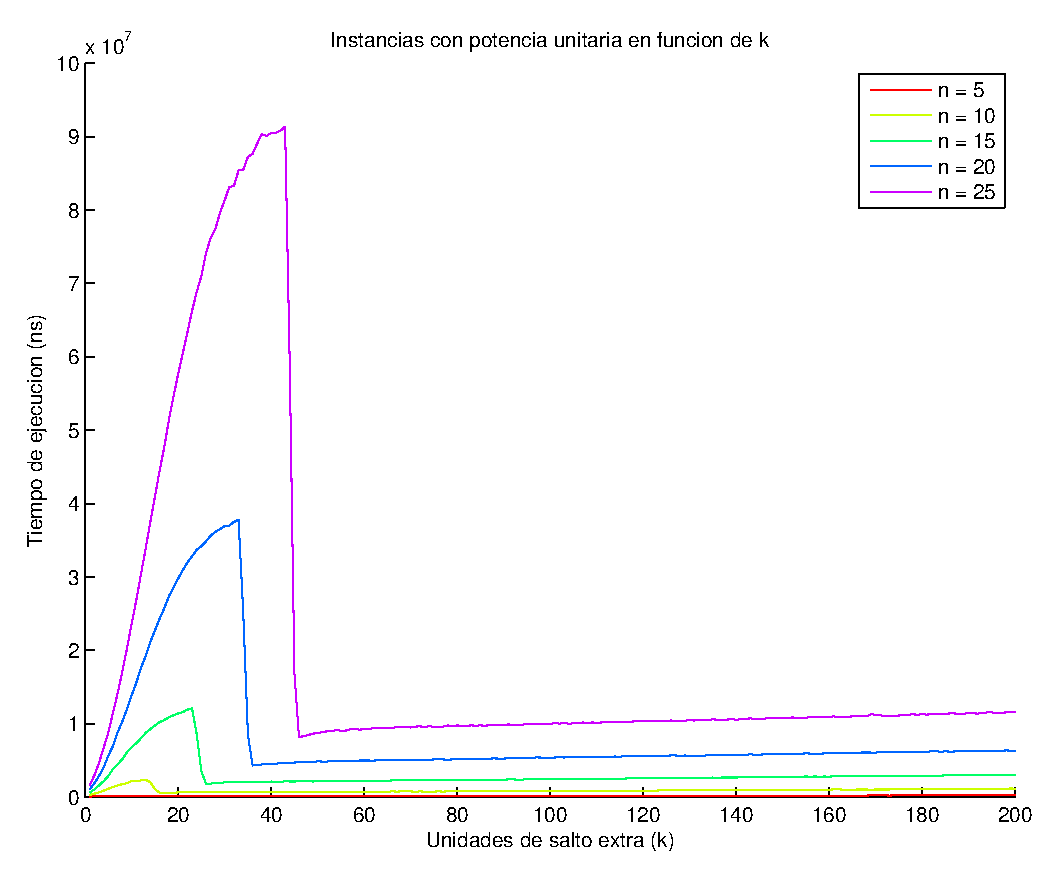
\includegraphics[width=\linewidth]{img/problema3/instancia_p_1_varios_n.eps}
    \caption{Tiempo de ejecución instancia aleatoria}\label{fig:problema3-n}
  \end{minipage}
  \hfill
  \begin{minipage}{0.5\linewidth}
    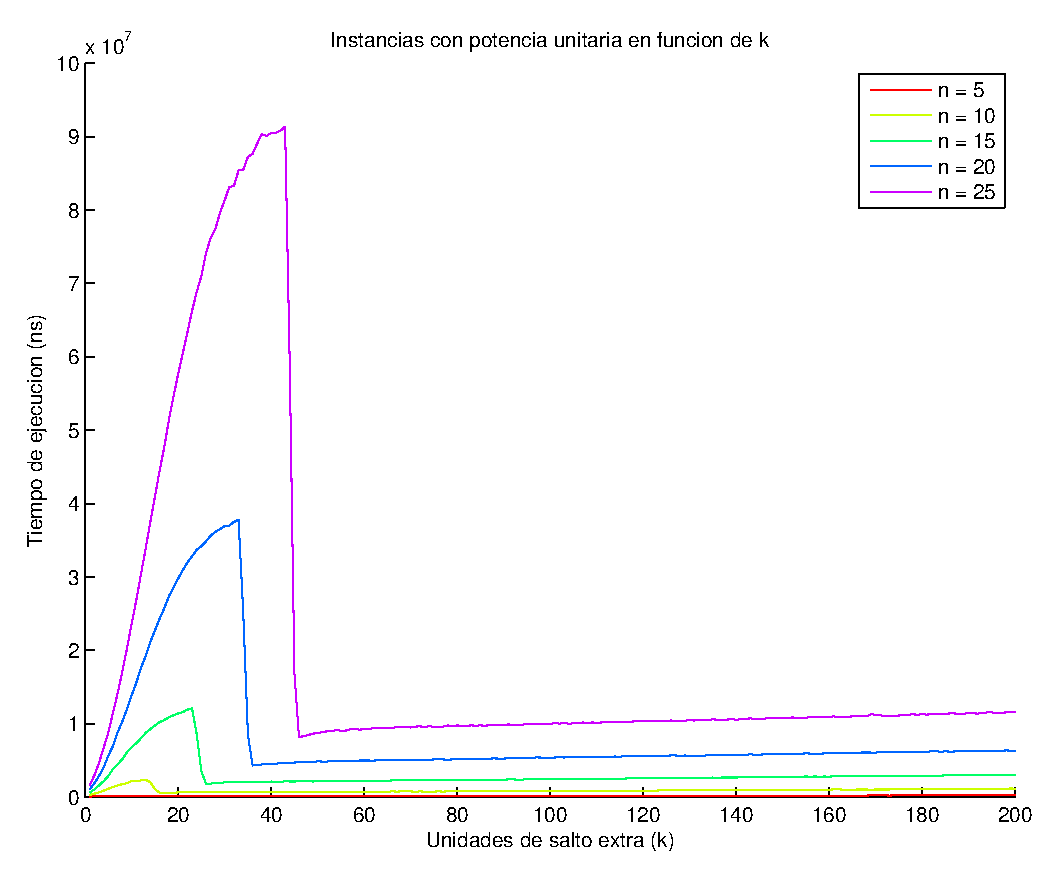
\includegraphics[width=\linewidth]{img/problema3/instancia_p_1_varios_n_div_n2.eps}
    \caption{Idem, dividido por $n^2$}\label{fig:problema3-n-n2}
  \end{minipage}
\end{figure}

En estos casos, una vez más podemos observar que cuando $k \geq 2*(n-2)$ resolver el problema es trivial. En estas figuras, está representado por la caída del tiempo de ejecución a partir de este punto. Cabe aclarar que si bien resolver el problema es trivial, al crecer el n cuesta más crear la matriz3D ya que la misma es más grande. Sin embargo, esta complejidad temporal es despreciable comparandola con $O(n^3*k)$.

Finalmente, decidimos probar un caso más: dejar fijo k y n, variando la potencia de los resortes.